\documentclass[11pt]{article}
\usepackage[T1]{fontenc}
\usepackage{lmodern,microtype}
\usepackage[margin=0.95in]{geometry}
\usepackage{amsmath,amssymb,amsthm,mathtools}
\usepackage{graphicx,booktabs,longtable,array,needspace}
\usepackage[dvipsnames]{xcolor}
\usepackage[colorlinks=true,linkcolor=MidnightBlue,citecolor=MidnightBlue,urlcolor=MidnightBlue]{hyperref}
\usepackage{fancyhdr}
\pagestyle{fancy}\fancyhf{}\fancyhead[L]{\small Geometric Flux and Magnetic Charge}\fancyhead[R]{\small Beasley, GPT, Claude}\fancyfoot[C]{\thepage}
\setlength{\headheight}{14pt}
\setlength{\parskip}{0.35em}
\setlength{\parindent}{0pt}
\setlength{\emergencystretch}{4em}
\newtheorem{theorem}{Theorem}[section]
\newtheorem{proposition}[theorem]{Proposition}
\newtheorem{corollary}[theorem]{Corollary}
\theoremstyle{definition}\newtheorem{definition}[theorem]{Definition}
\theoremstyle{remark}\newtheorem{remark}[theorem]{Remark}
\newcommand{\Tr}{\operatorname{Tr}}
\newcommand{\ii}{\mathrm{i}}
\newcommand{\dd}{\mathrm{d}}
\newcommand{\R}{\mathbb{R}}
\newcommand{\C}{\mathbb{C}}
\newcommand{\Z}{\mathbb{Z}}
\newcommand{\checked}{\textnormal{\small[Lean-checked components]}\ }
\newcommand{\written}{\textnormal{\small[Written proof; not formalized here]}\ }
\newcommand{\leanname}[1]{\texttt{\small\detokenize{#1}}}
\title{\vspace{-1.5em}From Geometric Flux to Magnetic Charge\\[0.4em]\large A Checked Pauli Curvature and an Explicit Physical Bridge}
\author{Jeromie Beasley \and GPT (OpenAI) \and Claude (Anthropic)}
\hypersetup{pdfauthor={Jeromie Beasley; GPT (OpenAI); Claude (Anthropic)}}
\date{Version 5.0 --- 5 November 2026\\\small Research note / draft for review}
\begin{document}
\maketitle
{\small\noindent\textbf{AI assistance.} Jeromie Beasley, GPT (OpenAI), and Claude (Anthropic) collaborated on the mathematics, drafting, Lean development, review and typesetting. GPT and Claude are AI systems. This draft has not been independently peer reviewed.\par}
\begin{abstract}
For the lower eigenprojector of the canonical two-level Pauli Hamiltonian, one Lean library now checks the full calculation from actual entrywise projector derivatives to curvature $\sin\theta/2$ and normalized flux $1$. An equality theorem joins the two matrix encodings, so the curvature derivation and flux integral are connected inside the proof system. Three further results sharpen the geometry: pole obstruction for a scalar primitive with equal pole values, latitude-cut independence for the fixed north and south coefficients, and derived band-flux cancellation for the complementary projector. The unified library contains 56 theorem declarations and rejects 11 deliberately false controls. We distinguish these checked statements from the standard written eigenline-bundle interpretation, general coordinate and gauge invariance, and pullback degree theory. A magnetic-charge conclusion additionally requires a spatial domain map and a physical identification such as $F_B=\kappa f^*\Omega$. The result is a continuous checked chain for this explicit example, with its mathematical and physical boundaries stated separately.

\end{abstract}
\noindent\textbf{Keywords:} Berry curvature; Pauli projector; magnetic monopole; first Chern number; physical identification; Lean 4.

\section{From a projector to a physical question}
Start with an eigenline that changes as the Hamiltonian changes. Its curvature records the geometry of that family. Integrating the curvature can retain an integer even though no magnetic field in physical space has yet been specified. The question is what carries that integer from one domain to the other.

The two-level Pauli example lets us follow each step explicitly: matrix, derivative, curvature, flux, and physical interpretation. This revision closes the earlier written join between the curvature calculation and its integral. Both now live in one pinned Lean library, with a theorem identifying the matrix encodings and a theorem integrating the curvature built from the actual derivatives.

The new results are pole obstruction, latitude-cut independence and derived band-flux cancellation. These names describe what the code proves. Together they explain why the fixed two-chart calculation retains one when the latitude cut moves, and why selecting the other band reverses it. General bundle topology gives the familiar coordinate-independent Chern interpretation; constructing that interpretation is a separate mathematical task.

The underlying geometry is classical. Dirac's construction concerns electromagnetic phase and magnetic charge \cite{dirac}; Berry and Simon describe eigenstate phase and line-bundle geometry \cite{berry,simon}; Wu and Yang explain the global connection picture \cite{wuyang}. The example also appears in the author's IQGT manuscript, Appendix B \cite{iqgt}. This note's contribution is a reproducible formal calculation and a clear account of the physical identification it needs.

We mark checked components and written proofs separately. The declaration map in Appendix~\ref{sec:map} gives the exact formal coverage. All physical interpretations use the domains, conventions and hypotheses stated below.

\section{Conventions and domains}
Let $\sigma_1,\sigma_2,\sigma_3$ be the standard Pauli matrices, satisfying
\begin{equation}\label{eq:pauli}
 (a\cdot\sigma)(b\cdot\sigma)=(a\cdot b)I+\ii(a\times b)\cdot\sigma,
 \qquad \Tr\sigma_j=0.
\end{equation}
For $d\in\R^3\setminus\{0\}$ write $n=d/|d|$ and consider
\begin{equation}\label{eq:h}
 H(d)=d\cdot\sigma,\qquad P_-(n)=\tfrac12(I-n\cdot\sigma).
\end{equation}
The base space at this stage is Hamiltonian \emph{parameter space}. On its unit sphere use
\begin{equation}\label{eq:n}
 n(\theta,\phi)=(\sin\theta\cos\phi,\sin\theta\sin\phi,\cos\theta),
 \quad 0\leq\theta\leq\pi,\quad 0\leq\phi<2\pi.
\end{equation}
The outward orientation is represented by $\dd\theta\wedge\dd\phi$ with its positive $\sin\theta$ surface density. For a normalized local eigenvector $u$, our Berry convention is
\begin{equation}\label{eq:berryconv}
 A=\ii u^\dagger\dd u,\qquad \Omega=\dd A,
 \qquad \Omega_{ab}=\ii\Tr\bigl(P_-[\partial_aP_-,\partial_bP_-]\bigr).
\end{equation}
Changing the sign convention for $A$, the band, or the orientation changes the corresponding sign. The nonvanishing statement is unaffected.

The magnetic two-form $F_B$ used later is a dimensionful physical quantity whose surface integral is magnetic flux. It is not defined to be $\Omega$. A coefficient converting between them must carry the requisite units, and a map must identify the parameter and spatial domains. We use $q_\Phi$ for a nonzero \emph{flux unit}; it is not an electric charge.

\section{Projector algebra and derived curvature}
\begin{proposition}[Pauli projector identities]\label{prop:projector}\checked
For real $x,y,z$ with $x^2+y^2+z^2=1$, the matrix
\begin{equation}\label{eq:pentries}
 P(x,y,z)=\frac12\begin{pmatrix}
 1-z&-x+\ii y\\-x-\ii y&1+z
 \end{pmatrix}
\end{equation}
is Hermitian and idempotent and has trace one.
\end{proposition}
\begin{proof}
Conjugation exchanges the off-diagonal entries. Put $N=n\cdot\sigma$. Equation~\eqref{eq:pauli} gives $N^2=I$, so
$P^2=(I-2N+N^2)/4=P$, and $\Tr P=1$.
The companion development proves these three matrix identities directly in fixed coordinates over $\C$; it does not rely on an assumed matrix identity named \eqref{eq:pauli}.
\end{proof}
In ordinary finite-dimensional spectral theory these identities specify an orthogonal rank-one projector. Moreover, $HP_-=-|d|P_-$ follows directly from~\eqref{eq:h}. The rank conclusion and this eigenvalue relation are written consequences here, not additional checked declarations.

\begin{proposition}[Berry curvature of the lower eigenline]\label{prop:curvature}\checked
With the convention~\eqref{eq:berryconv},
\begin{equation}\label{eq:omega}
 \Omega_{ab}=\tfrac12 n\cdot(\partial_a n\times\partial_b n),
 \qquad \Omega=\tfrac12\sin\theta\,\dd\theta\wedge\dd\phi.
\end{equation}
\end{proposition}
\begin{proof}
Set $a=\partial_a n$, $b=\partial_b n$, and $c=a\times b$. Differentiating $P_-=(I-n\cdot\sigma)/2$ and using~\eqref{eq:pauli} gives
\[
 [\partial_aP_-,\partial_bP_-]=\frac14[a\cdot\sigma,b\cdot\sigma]
 =\frac{\ii}{2}c\cdot\sigma.
\]
Since $\Tr((n\cdot\sigma)(c\cdot\sigma))=2n\cdot c$,
\[
 \Tr\bigl(P_-[\partial_aP_-,\partial_bP_-]\bigr)
 =-\frac{\ii}{2}n\cdot c.
\]
Multiplication by $\ii$ proves the first formula. For~\eqref{eq:n}, direct differentiation gives $\partial_\theta n\times\partial_\phi n=\sin\theta\,n$, yielding the second.
\end{proof}
The module \leanname{FluxCharge/Monopole.lean} checks this calculation in fixed $2\times2$ complex matrices. It proves the commutator for arbitrary real vectors, the exact increment
\[
 P(n+ha)-P(n)=hD(a),\qquad D(a)=-\tfrac12a\cdot\sigma,
\]
and the trace identity $\ii\Tr(P(n)[D(a),D(b)])=n\cdot(a\times b)/2$. Six \leanname{HasDerivAt} theorems identify the components of $\partial_\theta n$ and $\partial_\phi n$. The general lemma \leanname{hasDerivAt_proj_comp} differentiates every entry of the affine Pauli matrix formula along an arbitrary real path with differentiable components. Its two specializations \leanname{hasDerivAt_proj_theta} and \leanname{hasDerivAt_proj_phi} then prove, for every pair of matrix indices,
\[
 \frac{\dd}{\dd\theta}P(n(\theta,\phi))_{ij}=D(\partial_\theta n)_{ij},
 \qquad
 \frac{\dd}{\dd\phi}P(n(\theta,\phi))_{ij}=D(\partial_\phi n)_{ij}.
\]
These are derivatives of complex-valued entry functions, requiring no choice of a matrix norm. Finally, \leanname{berry_curvature_from_derivatives} builds the two derivative matrices entry by entry using Lean's \leanname{deriv} operator and proves that their matrix-trace curvature equals $\omega(\theta)=\sin\theta/2$. The derivative link and final trace calculation are thus joined by a checked theorem. The table transliterates the Unicode direction characters in the derivative theorem names. An exterior-form construction remains outside the module.

The module \leanname{FluxCharge/Seam.lean} now checks the identification. Its theorem \leanname{lowerProjector_eq_proj} equates the original explicit matrix with the matrix used in the derivative calculation. The theorem \leanname{proj_nvec_idempotent} then proves idempotence along the sphere. Define
\begin{equation}\label{eq:derived}
 C_-(\theta,\phi)=\Re\!\left(\ii\Tr\bigl(P_-[V,W]\bigr)\right),\quad
 V_{ij}=\frac{\dd}{\dd\theta}(P_-)_{ij},\quad
 W_{ij}=\frac{\dd}{\dd\phi}(P_-)_{ij}.
\end{equation}
Here the derivatives are Lean's actual \leanname{deriv} of complex-valued entry functions. The preceding complex trace theorem shows that the expression is already real. The theorem \leanname{derivedCurvature_eq} identifies $C_-$ with the same definition of $\omega$ used by the integral module; no equality between separately built projects is being assumed.

\begin{proposition}[Normalized flux]\label{prop:flux}\checked
Define the iterated coordinate flux and its normalization by
\begin{equation}\label{eq:fluxdef}
 \mathcal F(f)=\int_0^{2\pi}\!\dd\phi\int_0^\pi f(\theta)\,\dd\theta,
 \qquad \mathcal N(f)=\frac{\mathcal F(f)}{2\pi}.
\end{equation}
For $\omega(\theta)=\sin\theta/2$,
\begin{equation}\label{eq:unit}
 \int_0^\pi\omega(\theta)\,\dd\theta=1,\quad
 \mathcal F(\omega)=2\pi,\quad \mathcal N(\omega)=1\neq0.
\end{equation}
\end{proposition}
\begin{proof}
The first integral equals $[-\cos\theta/2]_0^\pi=1$. Integration in $\phi$ gives $2\pi$, and division by the nonzero number $2\pi$ gives one. Lean uses Mathlib's interval integral of sine and exact real arithmetic.
\end{proof}
For functions of two angular variables put
\begin{equation}\label{eq:coordflux}
 \mathcal C(F)=\int_0^{2\pi}\!\dd\phi\int_0^\pi F(\theta,\phi)\,\dd\theta.
\end{equation}
The theorem \leanname{coordFlux_eq_sphereFlux} identifies $\mathcal C((\theta,\phi)\mapsto f(\theta))$ with $\mathcal F(f)$. The theorem \leanname{derived_curvature_unit_flux} therefore proves
\begin{equation}\label{eq:derivedflux}
 \frac{\mathcal C(C_-)}{2\pi}=1.
\end{equation}
Finally, \leanname{matrix_to_integer} combines idempotence, the derived curvature coefficient, and~\eqref{eq:derivedflux} in one checked statement. The value one is an exact equality in $\R$. The theorem neither defines a Chern class nor proves that normalized flux is integer-valued for general families.

There is no additional surface Jacobian to insert into~\eqref{eq:fluxdef}: the coefficient in~\eqref{eq:omega} already contains $\sin\theta$. Multiplying it by another $\sin\theta$ would compute a different integral.

\section{Two charts and the meaning of the integer}
The familiar local eigenvectors make the geometric interpretation explicit. On the sphere with the south pole removed, and with the north pole removed, respectively, take
\begin{equation}\label{eq:states}
 u_N=\begin{pmatrix}-e^{-\ii\phi}\sin(\theta/2)\\\cos(\theta/2)\end{pmatrix},
 \qquad
 u_S=\begin{pmatrix}-\sin(\theta/2)\\e^{\ii\phi}\cos(\theta/2)\end{pmatrix}.
\end{equation}
They satisfy $H(n)u_{N,S}=-u_{N,S}$ and $u_S=e^{\ii\phi}u_N$ on the overlap. Computing~\eqref{eq:berryconv} gives
\begin{equation}\label{eq:charts}
 A_N=a_N(\theta)\,\dd\phi,\quad a_N=\frac{1-\cos\theta}{2};
 \qquad A_S=a_S(\theta)\,\dd\phi,\quad a_S=-\frac{1+\cos\theta}{2}.
\end{equation}
The apparent polar-coordinate singularity of $\dd\phi$ is cancelled by its coefficient at the included pole. The opposite pole is excluded from the respective chart. These are local descriptions of one connection, rather than one globally defined scalar potential on the entire sphere.

\begin{proposition}[Local coefficient identities]\label{prop:charts}\checked
For every real $\theta$,
\begin{equation}
 a_N'(\theta)=a_S'(\theta)=\omega(\theta),\qquad a_N(\theta)-a_S(\theta)=1.
\end{equation}
\end{proposition}
\begin{proof}
Differentiate~\eqref{eq:charts} and subtract the two coefficients. These scalar derivative and equality statements are precisely the checked claims.
\end{proof}
The line bundle assembled from~\eqref{eq:states} has the usual first-Chern interpretation
\begin{equation}\label{eq:chern}
 c_1[P_-]=\frac1{2\pi}\int_{S^2}\Omega=1
\end{equation}
with the specified convention. The transition phase on the equator has winding one. This is the standard eigenline-bundle interpretation, explained in writing using the local charts and classical connection theory \cite{simon,wuyang}. The companion code does not construct that bundle, its transition-function winding, or its Chern class. In particular, its name \leanname{normalizedFlux} denotes the real-valued expression in~\eqref{eq:fluxdef}, not a formal Chern-class definition.

\begin{figure}[t]
\centering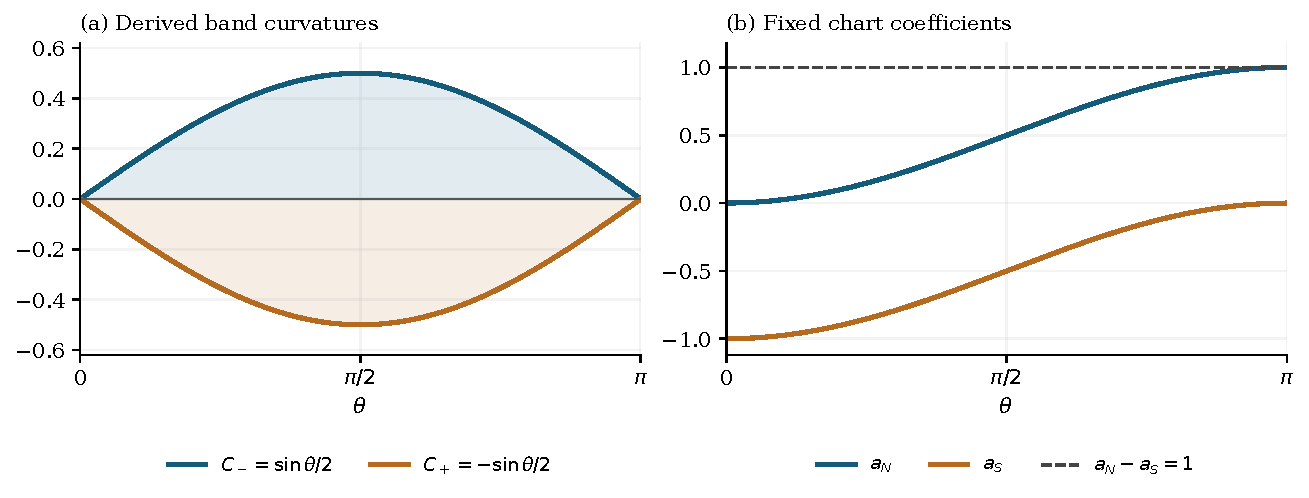
\includegraphics[width=\linewidth]{figures/curvature_and_gauges_v5.pdf}
\caption{Exact analytic functions in the two-level example. (a) The curvatures derived from the two projectors have polar integrals $+1$ and $-1$. (b) The fixed chart coefficients have equal derivatives and differ by one at every latitude. The north coefficient has pole values 0 and 1. These are analytic illustrations, not measured data; their scalar identities are checked in Lean.}
\label{fig:curvature}
\end{figure}

\subsection{Pole obstruction}
The pole values expose the obstruction at the level actually encoded by the library.
\begin{theorem}[Pole obstruction]\label{thm:pole}\checked
There is no $a:\R\to\R$ such that $a'(\theta)=\omega(\theta)$ for every real $\theta$ and $a(0)=a(\pi)$.
\end{theorem}
\begin{proof}
The derivative is continuous. The fundamental theorem of calculus and~\eqref{eq:unit} give
\[
 a(\pi)-a(0)=\int_0^\pi\omega(\theta)\,\dd\theta=1,
\]
contradicting equal endpoint values. This is \leanname{no_global_regular_gauge}.
\end{proof}
For the axisymmetric ansatz $A=a(\theta)\,\dd\phi$, smoothness at each pole requires its angular coefficient to vanish there. One way to see the necessary condition is to integrate a smooth one-form around shrinking latitude circles: the integrals tend to zero, whereas the ansatz gives $2\pi a(\theta)$. Thus a single smooth potential of this form would in particular have equal zero pole values, which the theorem excludes. This regularity argument is written geometry. The checked theorem quantifies over real functions and their derivatives, not arbitrary smooth one-forms on $S^2$.

The scalar functions $a_N$ and $a_S$ themselves are smooth for all real $\theta$. It is the regularity of $a\,\dd\phi$ on the sphere that requires attention. The result supports the two-patch construction; it does not assert that a physical Dirac string must exist. In ordinary bundle language the regular local potentials avoid a singular global-potential representation.

\subsection{Latitude-cut independence}
\begin{theorem}[Latitude-cut independence]\label{thm:cut}\checked
For every real cut $\theta_0$,
\begin{equation}\label{eq:cut}
 \int_0^{\theta_0}\omega\,\dd\theta+
 \int_{\theta_0}^{\pi}\omega\,\dd\theta
 =a_N(\theta_0)-a_S(\theta_0)=1.
\end{equation}
\end{theorem}
\begin{proof}
Use $a_N'=\omega$, $a_N(0)=0$ for the first integral and $a_S'=\omega$, $a_S(\pi)=0$ for the second. Their sum is $a_N(\theta_0)-a_S(\theta_0)$, which equals one. Lean proves the two equalities as \leanname{flux_is_transition_jump} and \leanname{flux_one_at_every_cut}.
\end{proof}
When $0\leq\theta_0\leq\pi$, the two terms are the normalized north- and south-cap contributions after azimuthal integration. Outside that interval, the same theorem is an oriented interval-integral identity. Moving the latitude cut leaves the sum fixed for the stated coefficients. This is narrower than invariance under arbitrary coordinate changes or arbitrary gauge transformations.

The standard topological interpretation comes from the transition phase $e^{\ii\phi}$ and its winding. A general local gauge change need not preserve a pointwise angular coefficient difference of one; the appropriate integrated transition invariant is the object that persists. The library checks the fixed coefficient identity and the cut-independent integral, while the transition map, its winding and the general invariance theorem remain written mathematics.

\section{Derived band-flux cancellation}
Let $P_+=I-P_-$. Define $C_+$ exactly as in~\eqref{eq:derived}, using the actual entrywise derivatives of $P_+$.
\begin{theorem}[Derived band-flux cancellation]\label{thm:bands}\checked
The complementary curvature and the two normalized fluxes satisfy
\begin{equation}\label{eq:bandflux}
 C_+(\theta,\phi)=-\frac{\sin\theta}{2},\qquad
 \frac{\mathcal C(C_+)}{2\pi}=-1,\qquad
 \frac{\mathcal C(C_-)}{2\pi}+\frac{\mathcal C(C_+)}{2\pi}=0.
\end{equation}
\end{theorem}
\begin{proof}
The checked theorems \leanname{hasDerivAt_compl_theta} and \leanname{hasDerivAt_compl_phi} differentiate every entry of $I-P_-$: the derivatives are the negatives of those of $P_-$. Their two minus signs cancel in the commutator. Since the trace of a commutator is zero,
\[
 \ii\Tr\bigl((I-P_-)[V,W]\bigr)
 =-\ii\Tr\bigl(P_-[V,W]\bigr).
\]
Lean combines the complement trace identity with the actual derivatives to prove \leanname{derivedCurvatureCompl_eq}. Integrating gives \leanname{derived_compl_flux}; combining it with~\eqref{eq:derivedflux} gives \leanname{total_chern_zero}.
\end{proof}
The last theorem's historical name is retained for compatibility. Its statement is a zero sum of normalized real integrals, not a theorem about a constructed Chern-class object. Standard bundle theory interprets the selected eigenlines as carrying opposite first Chern numbers in a trivial ambient two-band bundle. Cancellation of the sum leaves each selected-band contribution nonzero. This revision checks that cancellation from both projectors' actual derivatives, rather than merely integrating an independently supplied negative coefficient.

\section{An extension obstruction at the degeneracy}
At $d=0$, $H(d)$ has no isolated lower eigenline. The obstruction can be seen without any Chern-class machinery. Restricting the normalized direction to the $z$-axis gives
\begin{equation}\label{eq:axis}
 P_-(0,0,1)=\begin{pmatrix}0&0\\0&1\end{pmatrix},\qquad
 P_-(0,0,-1)=\begin{pmatrix}1&0\\0&0\end{pmatrix}.
\end{equation}
\begin{theorem}[No continuous axis extension]\label{thm:axis}\checked
Suppose $F:\R\to M_2(\C)$ satisfies $F(t)=P_-(0,0,1)$ for $t>0$ and $F(t)=P_-(0,0,-1)$ for $t<0$. Then $F$ is not continuous at zero.
\end{theorem}
\begin{proof}
The real part of its $(0,0)$ entry is zero on the positive half-axis and one on the negative half-axis. Along $t_m=1/(m+1)$ it tends to zero, and along $-t_m$ it tends to one. Both input sequences tend to zero. Continuity and uniqueness of limits would force $F(0)_{00}$ to have real part both zero and one, a contradiction. Lean proves the scalar jump obstruction and then applies it to the matrix coordinate.
\end{proof}
Any continuous three-dimensional extension of the normalized family that agrees with these axis values would restrict to such a continuous $F$; hence it cannot exist. That restriction argument and the three-dimensional spectral-family construction are stated in writing, while Theorem~\ref{thm:axis} is the exact checked result. This is a parameter-space degeneracy obstruction, not an electromagnetic source equation.

\section{The electromagnetic bridge}\label{sec:physical}
\subsection{A spatial domain and a map}
Let $\Sigma$ be a closed oriented physical spatial surface. A map $f:\Sigma\to S^2$ specifies how its points sample the Hamiltonian directions. It produces $f^*\Omega$, but this pullback is still an eigenstate-geometric two-form unless it is identified with the electromagnetic field measured by a stated probe.

A particularly transparent sufficient identification is
\begin{equation}\label{eq:physicalbridge}
 F_B\big|_\Sigma=\kappa f^*\Omega,
\end{equation}
where $\kappa$ is a nonzero dimensional coefficient. This equality is an additional hypothesis. A physical derivation must specify the coupling that makes the two curvatures the same observable, with consistent gauge transformations and normalization. Merely giving both quantities a connection or curvature notation does not supply that derivation.

\begin{proposition}[Conditional pullback flux]\label{prop:pullback}\written
If $\Sigma\simeq S^2$, $f$ is smooth of degree $d$, and~\eqref{eq:physicalbridge} holds, then
\begin{equation}\label{eq:degreeflux}
 \Phi_B:=\int_\Sigma F_B=2\pi\kappa d.
\end{equation}
More generally, put $n=(2\pi)^{-1}\int_\Sigma f^*\Omega$ whenever this record is justified. Then $\Phi_B=q_\Phi n$ with $q_\Phi=2\pi\kappa$.
\end{proposition}
\begin{proof}
The integral of the pullback of an oriented top-degree form under a smooth sphere map multiplies the integral by its degree. Apply that standard degree formula to~\eqref{eq:unit} and multiply by $\kappa$. The second assertion is substitution. Neither the degree formula nor the pullback construction is formalized in the unified library.
\end{proof}
A constant map has $d=0$, even though the original parameter-sphere eigenline has $c_1=1$. An orientation-preserving degree-one map retains the unit normalized flux. Specifying a domain map is therefore essential even before specifying the electromagnetic coupling.

For a probe of nonzero signed electric charge $e$, a conventionally compatible physical identification of its dimensionless connection can set $\kappa=\hbar/e$. Under that \emph{additional identification},~\eqref{eq:degreeflux} reads $\Phi_B=(h/e)d$. This illustrates the usual Dirac flux unit; it neither derives the identification from the two-level projector nor reports an observed monopole. We keep flux separate from magnetic-source conventions that introduce factors such as $\mu_0$.

\subsection{An explicit exterior field}
As a written example on punctured Euclidean space, choose $f(x)=x/|x|$ and impose~\eqref{eq:physicalbridge}. The associated radial magnetic field is
\begin{equation}\label{eq:radial}
 B(x)=\frac{\kappa}{2}\frac{\widehat x}{|x|^2},\qquad x\neq0.
\end{equation}
Its flux is $2\pi\kappa$ through every centered sphere. This is the standard monopole exterior geometry, smooth away from the missing origin. It is a valid mathematical example conditional on the imposed field identification; it does not provide a nonsingular core, a source dynamics, or an empirical realization.

The exact formalized calculation is narrower. For the supplied unit-sphere density $g\sin\theta$, Lean proves
\begin{equation}\label{eq:radialflux}
 \mathcal F(g\sin\theta)=4\pi g,\qquad
 \mathcal F(g\sin\theta)\neq0\ \Longleftrightarrow\ g\neq0.
\end{equation}
Taking $g=\kappa/2$ reproduces the flux of~\eqref{eq:radial}. The code does not construct a spatial vector field or prove its Maxwell equations.

\section{Charge transfer with an explicit bridge}
A small numerical model isolates the role of the bridge.
\begin{definition}[Charge record]\label{def:record}
A record is a pair $r=(n,\Phi)\in\Z\times\R$. Write
\[
 G(r)\ \Longleftrightarrow\ n\neq0,\qquad
 M(r)\ \Longleftrightarrow\ \Phi\neq0.
\]
For a specified flux unit $q_\Phi$, define the bridge predicate
\begin{equation}\label{eq:recordbridge}
 E(q_\Phi,r)\ \Longleftrightarrow\ \Phi=q_\Phi n.
\end{equation}
\end{definition}
Here $n$ is supplied as an integer; the type itself proves no integrality theorem. The code uses ``magnetically charged'' to mean $\Phi\neq0$. The physical meaning of $\Phi$ comes from the preceding spatial and field identification.

\begin{theorem}[Counterassignments without a bridge]\label{thm:counter}\checked
For every integer $n$, the records $r_0=(n,0)$ and $r_1=(n,1)$ have the same geometric coordinate, while $\neg M(r_0)$ and $M(r_1)$. In particular,
\begin{align}
 \neg\bigl(\forall r,\ G(r)\Rightarrow M(r)\bigr),\\
 \neg\bigl(\forall r,\ G(r)\Rightarrow\neg M(r)\bigr).
\end{align}
\end{theorem}
\begin{proof}
The first assertion is immediate from the coordinates. Taking $n=1$ gives a counterexample to either universal implication. Lean supplies these explicit witnesses.
\end{proof}
The records $(1,0)$ and $(1,1)$ demonstrate that two freely assigned coordinates carry no relation until one is imposed. They are numerical witnesses, not physical solutions. Their purpose is to locate the missing premise.

\begin{theorem}[Charge transfer under the bridge]\label{thm:transfer}\checked
If $q_\Phi\neq0$ and $E(q_\Phi,r)$, then
\begin{equation}\label{eq:iff}
 M(r)\ \Longleftrightarrow\ G(r).
\end{equation}
\end{theorem}
\begin{proof}
Substitute $\Phi=q_\Phi n$. Since $\R$ has no zero divisors, $q_\Phi n\neq0$ is equivalent to $n\neq0$ when $q_\Phi\neq0$. The embedding $\Z\hookrightarrow\R$ preserves zero. These are the steps checked by \leanname{bridge_transfers_charge}.
\end{proof}
The arithmetic is elementary. The physical work lies in deriving the bridge for the system and probe under study.

Two useful companion facts are checked. First, a unit geometric record with zero magnetic flux cannot satisfy a nonzero-unit bridge. Second, for any chosen $q_\Phi$ and $n$ there exists the numerical bridge-compatible record $(n,q_\Phi n)$. These are consistency checks for the numerical definitions.

\section{The limits of a no-flux argument}
There is also a precise boundary to an absence claim. If a globally defined smooth one-form $A$ exists on a closed oriented surface $\Sigma$ and $F_B=\dd A$ there, Stokes' theorem gives $\int_\Sigma F_B=0$. Likewise, if a smooth closed field extends over a ball bounded by $\Sigma$, its boundary flux vanishes. These are written standard differential-form arguments, not theorems in this Lean package.

Their hypotheses matter. A nontrivial line bundle may require local potentials, and a punctured ball need not admit the extension required by the second argument. Local closedness $\dd F_B=0$ on the punctured exterior does not force all closed-surface fluxes there to vanish. The local charts in Section~4 demonstrate how a nonzero curvature integral can coexist with regular potentials on separate patches.

The code isolates the simplest logical version. Let $A_0(r)$ mean $\Phi=0$. It proves
\begin{equation}\label{eq:admiss}
 (\forall r,\ A_0(r)\Rightarrow\neg M(r))
 \quad\text{and}\quad
 \neg(\forall r,\neg M(r)).
\end{equation}
The first statement restricts an admitted class. The second uses a record outside that class. Thus imposing zero flux as an admissibility condition is different from deriving a universal no-monopole theorem. The numerical statement isolates the distinction between restricting a class and deriving a property of every member of a physical theory.

\section{Relation to projector transport and retained information}
The example illustrates a methodological point relevant to a transport atlas: identify the object, base space and observation before treating two invariants as the same quantity. Several distinctions are already visible in this note.

\begin{center}\small
\begin{tabular}{p{0.23\linewidth}p{0.31\linewidth}p{0.36\linewidth}}
\toprule
Record & What it retains here & What it does not supply by itself\\\midrule
Selected projector $P_-$ & An eigenline at each parameter point & A physical spatial map or EM coupling\\
Scalar curvature integral & One oriented normalized flux & The full local field or dynamics\\
Summed two-band curvature & Cancellation of opposite contributions & Vanishing of each selected-band contribution\\
Geometric integer $n$ & One topological/flux label under stated assumptions & A dimensional magnetic-flux unit\\
Candidate spatial flux $\Phi$ & An integrated physical reading once identified & A core solution, particle mass or production mechanism\\\bottomrule
\end{tabular}
\end{center}
A scalar summary can discard a distinction retained by a selected sector. Here the most immediate example is cancellation of two nonzero band fluxes in a trivial ambient bundle. That observation supports careful record selection; it does not identify Berry curvature, Hopf charge, instanton number or spectral flow with the same electromagnetic magnetic charge. Nor does the name ``monopole'' for an isotropic angular moment in a transport expansion perform such an identification.

For a light-transport, black-hole or neutrino model, the same discipline applies: specify the base space, retained sector, observable map and coupling before transferring an invariant. The present example supplies a worked template for that step.

\section{Formal verification and reproducibility}\label{sec:formal}
The current proof chain is one library, \leanname{FluxCharge}, pinned to Lean 4.34.1 and Mathlib v4.34.1. The repository is separate from the IQGT project. Its inventory is:
\begin{center}
\begin{tabular}{lr}
\toprule Module & Theorem declarations\\\midrule
\leanname{FluxCharge.Monopole} & 17\\
\leanname{FluxCharge.Geometry} & 13\\
\leanname{FluxCharge.Bridge} & 9\\
\leanname{FluxCharge.Extension} & 2\\
\leanname{FluxCharge.Seam} & 6\\
\leanname{FluxCharge.Topology} & 9\\\midrule
Total & 56\\\bottomrule
\end{tabular}
\end{center}
The 56 count theorem declarations, not definitions or 56 independent discoveries. The original 24 are included through their port. They must not be added again. All declarations retain the namespace \leanname{MonopoleStance}.

The check builds the library, independently replays all six modules using \leanname{leanchecker}, and audits every named theorem. Only \leanname{propext}, \leanname{Classical.choice} and \leanname{Quot.sound} are permitted dependencies. A fixed inventory in \leanname{scripts/config.json} requires exactly 56 theorems and 11 false controls. The controls target zero unit flux; either unconditional magnetic inference; a zero bridge unit; idempotence at the origin; zero chart-coefficient difference; the missing curvature factor one half; the wrong derivative sign; doubled derived flux; equal north-coefficient pole values; and a total band flux of two. The script distinguishes mathematical rejection from failures due to missing imports or unknown identifiers. Rejection exercises these attempted false proofs; it is not a general completeness guarantee for the verifier.

The proof-source revision is \href{https://github.com/dicipler-pixel/geometric-flux-magnetic-charge-lean/commit/d02b612e508e083e94baaf7d781ef15b76953f68}{\texttt{d02b612}} on branch \leanname{v5-seam}. Its \href{https://github.com/dicipler-pixel/geometric-flux-magnetic-charge-lean/actions/runs/42027723304}{successful CI run} records the build, independent kernel replay, axiom audit and all 11 rejected controls. The source snapshot and verification evidence accompany this paper. From the repository root, reproduce the unified check with \leanname{lake exe cache get}, \leanname{lake build}, and \leanname{python3 scripts/verify.py}; the workflow supplies the independent replay command.

The unchanged historical project remains under \leanname{monopole_stance/}, pinned separately to Lean 4.19.0 and its original Mathlib lock file. CI also rebuilds and audits that 24-theorem archive with its six controls. This preserves provenance; the archived project is not needed to fill a gap in the current unified chain. The earlier IQGT branch and its unrelated repository-wide counts belong to the development history, not the v5 theorem inventory.

\section{What the checked calculation adds}
The complete checked calculation starts with the explicit projector, differentiates its entries, computes the curvature, identifies that coefficient with the integral module's definition, and obtains normalized flux one. Pole obstruction and latitude-cut independence then expose the fixed local-coefficient structure. Repeating the derivative calculation for the complementary band gives normalized flux minus one and exact cancellation.

The boundaries now have specific mathematical targets. First, construct the global eigenline bundle, its transition map and Chern class, and identify that class with the normalized curvature integral. This would turn the written topological interpretation into a checked one. Second, prove the appropriate invariance under general coordinate and gauge changes; moving the latitude cut alone is not that theorem. Third, construct spatial pullbacks and their degree formula. Finally, derive the physical field identification for a stated system and probe. That last step requires physical input even if all the preceding geometry is formalized.

The present calculation concerns the canonical degree-one Pauli sphere. A general smooth gapped two-level family can wrap that sphere with a different degree, including zero. Nonzero gap alone does not force unit flux. Neither a coordinate value of one nor the numerical bridge records assert the existence or absence of a magnetic particle.

For the transport atlas, the practical rule is precise: keep the invariant with its domain and observation map. Berry flux, Hopf charge, instanton number and an $\ell=0$ transport moment can each be useful while retaining different meanings. A successful bridge identifies the relevant structures and units in a particular system. That is where a geometric calculation becomes a testable magnetic-field claim.

\clearpage
\appendix
\section{Complete declaration-to-claim map}\label{sec:map}
All names below lie in the namespace \leanname{MonopoleStance}. The first table lists the 24 ported declarations. The second lists the 17 projector-derivation declarations. The final table lists the 15 declarations that join the chain and add the new results. Together these are all 56 theorem declarations in the unified library. Local eigenvector chart construction, the Chern-class interpretation, physical pullbacks and Stokes arguments remain written mathematics.

\begin{longtable}{p{0.49\linewidth}p{0.45\linewidth}}
\toprule\textbf{Lean declaration} & \textbf{Exact role}\\\midrule\endfirsthead
\toprule\textbf{Lean declaration} & \textbf{Exact role}\\\midrule\endhead
\multicolumn{2}{l}{\textbf{Geometry: 13 declarations}}\\
\leanname{lowerProjector_hermitian} & Hermiticity of the explicit matrix.\\
\leanname{lowerProjector_idempotent} & Idempotence under unit-norm hypothesis.\\
\leanname{lowerProjector_trace} & Trace equals one.\\
\leanname{omega_polar_integral} & Polar integral of supplied coefficient equals one.\\
\leanname{omega_sphereFlux} & Iterated flux equals $2\pi$.\\
\leanname{omega_unit_normalizedFlux} & Normalized flux equals one.\\
\leanname{omega_nonzero_normalizedFlux} & Same normalized flux is nonzero.\\
\leanname{opposite_flux_cancels} & Supplied opposite coefficients have cancelling integrals.\\
\leanname{north_derivative} & Derivative of $a_N$ equals $\omega$.\\
\leanname{south_derivative} & Derivative of $a_S$ equals $\omega$.\\
\leanname{gauge_coefficient_difference} & $a_N-a_S=1$.\\
\leanname{radialFlux_eq} & Supplied radial density integrates to $4\pi g$.\\
\leanname{radialFlux_nonzero_iff} & That flux is nonzero exactly when $g\neq0$.\\\midrule
\multicolumn{2}{l}{\textbf{Extension: 2 declarations}}\\
\leanname{no_continuous_jump_extension} & Distinct constant half-axis values preclude continuity.\\
\leanname{no_continuous_Pauli_axis_extension} & Matrix application using the two pole projectors.\\\midrule
\multicolumn{2}{l}{\textbf{Bridge: 9 declarations}}\\
\leanname{bridge_transfers_charge} & Nonzero-unit bridge transfers nonzero charge.\\
\leanname{same_geometry_opposite_magnetic_status} & Same geometric coordinate; zero and unit flux.\\
\leanname{unit_geometry_compatible_with_both_records} & Both assignments at geometric charge one.\\
\leanname{no_unconditional_existence_inference} & Counterexample to universal existence inference in the record language.\\
\leanname{no_unconditional_absence_inference} & Counterexample to universal absence inference in the record language.\\
\leanname{unit_geometry_zero_flux_excludes_bridge} & Unit geometry and zero flux exclude a nonzero-unit bridge.\\
\leanname{bridge_record_exists} & Numerical record $(n,q_\Phi n)$ exists.\\
\leanname{admissibility_is_restriction} & Zero-flux restriction does not cover all records.\\
\leanname{formal_stance} & Conjunction of unit flux, both assignments and conditional transfer.\\\bottomrule
\end{longtable}

\Needspace{6\baselineskip}
\subsection*{Matrix-curvature module: 17 declarations}
\begin{longtable}{p{0.49\linewidth}p{0.45\linewidth}}
\toprule\textbf{Lean declaration} & \textbf{Exact role}\\\midrule\endfirsthead
\toprule\textbf{Lean declaration} & \textbf{Exact role}\\\midrule\endhead
\leanname{pauli_comm} & Pauli commutator for arbitrary real vectors.\\
\leanname{proj_affine} & Exact affine increment of the projector matrix.\\
\leanname{curvature_formula} & Matrix-trace curvature identity.\\
\leanname{hasDerivAt_nvec_theta1} & First component of $\partial_\theta n$.\\
\leanname{hasDerivAt_nvec_theta2} & Second component of $\partial_\theta n$.\\
\leanname{hasDerivAt_nvec_theta3} & Third component of $\partial_\theta n$.\\
\leanname{hasDerivAt_nvec_phi1} & First component of $\partial_\phi n$.\\
\leanname{hasDerivAt_nvec_phi2} & Second component of $\partial_\phi n$.\\
\leanname{hasDerivAt_nvec_phi3} & Third component of $\partial_\phi n$.\\
\leanname{hasDerivAt_proj_comp} & Entrywise chain rule along any real path with differentiable components.\\
\leanname{hasDerivAt_proj_theta} & Actual derivative of each projector entry in $\theta$.\\
\leanname{hasDerivAt_proj_phi} & Actual derivative of each projector entry in $\phi$.\\
\leanname{berry_curvature_from_derivatives} & Curvature built from actual entrywise derivatives.\\
\leanname{triple_product} & Spherical triple product equals $\sin\theta$.\\
\leanname{berry_curvature} & Trace coefficient equals $\omega(\theta)$.\\
\leanname{berry_curvature_eq_zero_iff} & $\omega(\theta)=0$ iff $\sin\theta=0$.\\
\leanname{complement_curvature} & Complementary matrix has opposite curvature.\\\bottomrule
\end{longtable}

The eight direction-labelled derivative names use the Unicode characters $\theta$ and $\phi$ in the Lean source; the table transliterates them for PDF font compatibility.

\Needspace{6\baselineskip}
\subsection*{Unified join and new results: 15 declarations}
\begin{longtable}{p{0.49\linewidth}p{0.45\linewidth}}
\toprule\textbf{Lean declaration} & \textbf{Exact role}\\\midrule\endfirsthead
\toprule\textbf{Lean declaration} & \textbf{Exact role}\\\midrule\endhead
\multicolumn{2}{l}{\textbf{Seam: 6 declarations}}\\
\leanname{lowerProjector_eq_proj} & Equality of the two explicit matrix encodings.\\
\leanname{proj_nvec_idempotent} & Idempotence along the spherical direction map.\\
\leanname{derivedCurvature_eq} & Actual derivative curvature equals the shared $\omega$.\\
\leanname{coordFlux_eq_sphereFlux} & Equality of the two coordinate-integral definitions.\\
\leanname{derived_curvature_unit_flux} & Actual derivative curvature has normalized real flux one.\\
\leanname{matrix_to_integer} & Conjunction of idempotence, derived coefficient and real flux one.\\
\midrule\multicolumn{2}{l}{\textbf{Topology: 9 declarations}}\\
\leanname{continuous_omega} & Continuity of the scalar curvature coefficient.\\
\leanname{no_global_regular_gauge} & No real primitive of $\omega$ has equal pole endpoint values.\\
\leanname{flux_is_transition_jump} & Split polar integral equals the fixed coefficient difference.\\
\leanname{flux_one_at_every_cut} & Split polar integral equals one at every real cut.\\
\leanname{hasDerivAt_compl_theta} & Actual $\theta$ derivative of every complementary-projector entry.\\
\leanname{hasDerivAt_compl_phi} & Actual $\phi$ derivative of every complementary-projector entry.\\
\leanname{derivedCurvatureCompl_eq} & Complementary curvature from actual derivatives equals $-\omega$.\\
\leanname{derived_compl_flux} & Complementary normalized real flux equals minus one.\\
\leanname{total_chern_zero} & Sum of normalized real fluxes is zero; no Chern-class object.\\
\bottomrule
\end{longtable}
The two complementary-projector derivative names likewise use Unicode $\theta$ and $\phi$ in the source. Transliteration changes display only; the proof snapshot preserves the exact identifiers.

\section{Combined formal statement}
The record-language theorem \leanname{formal_stance}, inherited from the original package, is
\begin{align*}
 &\mathcal N(\omega)=1\\[-0.3em]
 &\quad\land\bigl[(\exists r:\ n(r)=1\land\neg M(r))
       \land(\exists r:\ n(r)=1\land M(r))\bigr]\\[-0.3em]
 &\quad\land\bigl[\forall q_\Phi\neq0\ \forall r:\
 E(q_\Phi,r)\Rightarrow(M(r)\Longleftrightarrow G(r))\bigr].
\end{align*}
The first conjunct concerns a real integral. The second concerns freely assigned records. No formal map from that integral to the integer field of a record is asserted by the conjunction. In the physical application that interpretation is an additional construction, discussed in Section~4 and Section~\ref{sec:physical}. The separate \leanname{matrix_to_integer} theorem now connects the actual matrix derivatives to the real integral, but it still constructs no map to the record's integer field. The third conjunct is a transfer implication given a bridge. Reading all three as one unconditional physical-existence theorem would erase their different domains and hypotheses.

\section*{Data, code and assistance}
No experimental dataset is introduced. Figure~\ref{fig:curvature} plots analytic formulas. The companion source, locked build configuration, verification script and logs are supplied with this draft. The contributor names and AI disclosure appear above the abstract. The unified source snapshot and exact CI evidence accompany the unchanged original proof archive. The independent symbolic checks of the written formulas supplement, rather than replace, the Lean checks.

\clearpage
\begin{thebibliography}{9}
\bibitem{dirac} P. A. M. Dirac, ``Quantised singularities in the electromagnetic field,'' \emph{Proc. R. Soc. Lond. A} \textbf{133}, 60--72 (1931). \href{https://doi.org/10.1098/rspa.1931.0130}{doi:10.1098/rspa.1931.0130}.
\bibitem{berry} M. V. Berry, ``Quantal phase factors accompanying adiabatic changes,'' \emph{Proc. R. Soc. Lond. A} \textbf{392}, 45--57 (1984). \href{https://doi.org/10.1098/rspa.1984.0023}{doi:10.1098/rspa.1984.0023}.
\bibitem{simon} B. Simon, ``Holonomy, the quantum adiabatic theorem, and Berry's phase,'' \emph{Phys. Rev. Lett.} \textbf{51}, 2167--2170 (1983). \href{https://doi.org/10.1103/PhysRevLett.51.2167}{doi:10.1103/PhysRevLett.51.2167}.
\bibitem{wuyang} T. T. Wu and C. N. Yang, ``Concept of nonintegrable phase factors and global formulation of gauge fields,'' \emph{Phys. Rev. D} \textbf{12}, 3845--3857 (1975). \href{https://doi.org/10.1103/PhysRevD.12.3845}{doi:10.1103/PhysRevD.12.3845}.
\bibitem{iqgt} J. Beasley, \emph{Intrinsic Quantum Geometric Tensor on the Grassmannian and Spectral Lower Bounds on Dissipation}, version 7.3.1, author manuscript (2026), Appendix B. Supplied manuscript source; no archival identifier is asserted here.
\bibitem{lean} Lean development team, \emph{Lean 4}, version 4.34.1, \url{https://github.com/leanprover/lean4/releases/tag/v4.34.1}. Exact compiler identification is recorded in the companion verification log.
\bibitem{mathlib} Mathlib contributors, \emph{Mathlib}, version v4.34.1, \url{https://github.com/leanprover-community/mathlib4/tree/v4.34.1}. The companion lock file specifies the complete dependency graph.
\end{thebibliography}
\end{document}

